\chapter{Appendix}
\label{sec:appendix}

\section{Glacier marriage ceremony}
\label{sec:glacier_marriage}

This description of the glacier marriage ceremony is adapted from \citet{khanMarriageGlaciersPrzekroj2020}.

A 12-man party carries the pieces of female ice in woven baskets, another 12 men carry the male ice, the water
drawn from the Indus river is carried traditionally in 12 gourd bottles, but sometimes clay pots or goatskins
are also required, as well as charcoal and wheat husks or sawdust which act as insulators for the ice. The last
ingredient is salt, which, according to some glacier grafters, helps protect the new glacier from impurities.
The bride and groom party walk from different sites and meet at a certain point to climb together to their
destination, where the new glacier will be created. No greetings are exchanged, as the people involved in the
ceremony must remain silent until the ice is deposited in its new home. They walk continuously without
any breaks, but if the distance is too much and rest is required, they do not put their loads on the ground:
Instead, they hang the baskets on trees, or on walking sticks if nothing else is available. Each man has to
carry around 15 to 25 kilograms of ice, walking in cold air, silently up the mountains, for a day or more. Once
they reach the glacier growing site, they deposit their valuable loads. The ice lumps and water vessels are
placed in between the boulders, or in a small cave, or sometimes in a pit dug specifically for this purpose, and
are covered with layers of salt, charcoal and sawdust. The silence is finally broken as religious leaders recite
verses of the Quran and pray for the success of the glacier marriage and for protection from the djinns. Once
the male and female glaciers are placed in their new home and covered, a man from the glacier grafters' party
stands up and offers his life for the success of the process. His symbolic sacrifice is matched by the actual
sacrifice of a goat – its meat is distributed to a charity, because prayers are more likely to be answered if
accompanied by a charitable act. They will not visit the place for at least three years, so as not to disturb
the glacier. It is said that a person who disturbs the glacier before its maturation will die. The celebrations
continue in the village with traditional songs and prayers, alongside festive food and the joy of the
accomplished mission.


\section{Drone surveys processing methodology}
\label{sec:drone_method}

The drone flew along a predefined flight course and took photographs at a set time interval. The
position and altitude of the drone at the exposure stations, which were obtained by the built-in integrated
Position and Orientation System (POS, composed of a global positioning system and inertial measurement units),
were recorded in JPEG pictures. In this study, we adopted a three-step workflow as implemented in the
commercial software package Pix4Dmapper version 4.6.4 (\cite{pix4dsaPix4DmapperUserManual2020}). A short summary of this workflow is
described below:

\begin{figure}
	\begin{center}
		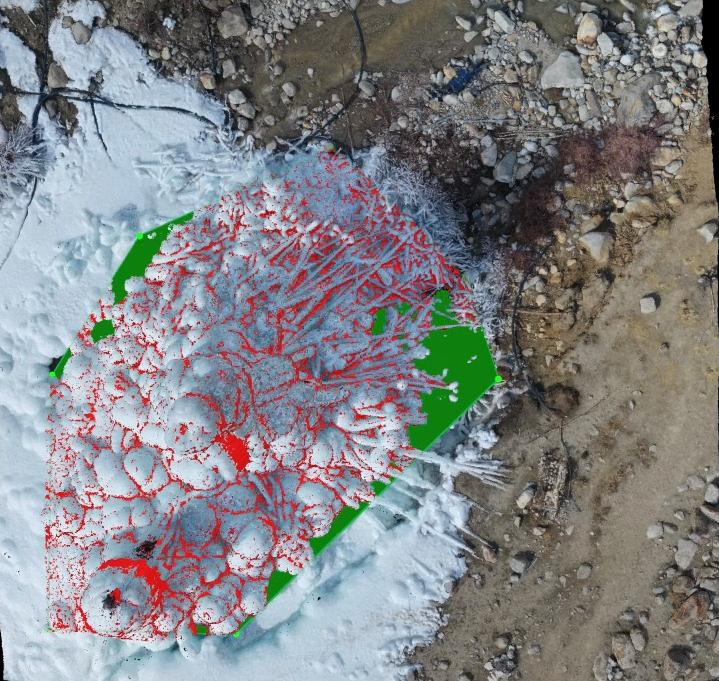
\includegraphics[width=12 cm]{figs/pix4d.jpg}
	\end{center}
	\caption{Digital elevation map of Indian AIR constructed from the drone survey on March 3, 2021. The green
		area represents the area bounded by the marked perimeter and the red area represents gaps in the point cloud
    that were filled to compute the associated volume.
	}
	\label{fig:DEM}
\end{figure}

(1) Initial processing: This process generates a sparse point cloud with the structure-from motion algorithm
(\cite{turnerAutomatedTechniqueGenerating2012}). First, it searches for and matches key points in the photos that have certain overlapping
areas using a feature matching algorithm (e.g., the scale-invariant feature transform (SIFT) algorithm, which can
detect key points in photos with different views and illumination conditions;
\cite{loweDistinctiveImageFeatures2004}). Second, the approximate locations and orientations of the camera at
each exposure station are reconstructed with the internal parameters (focal length, coordinates of the principal
point of the photograph), and external parameters (i.e. POS data). A sparse point cloud is created.

(2) Point cloud densification: In this step, the multi-view stereo technique is applied to achieve a higher
point cloud density than in the previous step (\cite{furukawaAccurateDenseRobust2010};
\cite{molgStructurefromMotionUsingHistorical2017}). Thus, the spatial resolution of the products can be
increased, and an irregular network for the next step can be created (\cite{kungACCURACYAUTOMATICPHOTOGRAMMETRIC2011}).

(3) AIR delineation: Ice radius, area and volume are the three final products. Perimeter was manually marked
on the point cloud by identifying the AIR boundary (see Fig. \ref{fig:DEM}). For the Indian location, we identified identical rock features
near the ice boundary to mark as vertices of this perimeter. For the Swiss AIR, no such feature was available due
to snowfall, so instead the perimeter was marked by identifying the ice and snow boundary.

There is temporal and spatial uncertainty associated with this process. Weather conditions influence the quality
of each drone survey to various degrees. Moreover, since ice/snow surfaces do not have many identifiable features, few
feature points can be detected and matched in the vicinity of the AIR. Thus, we attach a high uncertainty of
$\pm 10 \%$ for all the AIR observations to accommodate for this.

\begin{table}[htb]
  \centering
  \caption{List of all the studied AIRs in Ladakh. Adapted from \citet{mariagruberIceStupasLadakh2022}}
	\label{tab:Ladakh_AIRs}
	\begin{tabular}{|lllll|}
    \hline
    \textbf{Location}     & \textbf{Winter season} & \textbf{Altitude [$m\,a.s.l.$]} & \textbf{
    Radius [$m$]} & \textbf{Volume [$m^3$]} \\ \hline
    Igoo & 2019--20 & 4209 & 23 & 4918  \\
    Karith & 2019--20 & 3710 & 12 & 1451  \\
    Karith 2 & 2020--21 & 3692 & 5 & 1133  \\
    Lamso & 2019--20 & 3859 & 7 & 615  \\
    Lamso 2& 2020--21 & 3863 & 6 & 420  \\
    Nang& 2019--20 & 3897 & 13 & 1601 \\
    Phyang& 2019--20 & 3916 & 19 & 5182 \\
    Sandoo& 2019--20 & 3773 & 10 & 1483 \\
    Shara& 2019--20 & 4288 & 18 & 7936 \\
    Gangles& 2020--21 & 4072 & 9 & 602 \\
    Apati& 2020--21 & 3840 & 6 & 351 \\
    Mulbeck& 2019--20 & 3451 & 11 & 1887\\
    Nang& 2019--20 & 3897 & 13 & 1601\\
    Skurbuchan& 2019--20 & 3023 & 9 & 956\\
    Takmachik& 2019--20 & 3032 & 13 &1265\\
    Takmachik 2& 2020--21 & 3052 & 10 &1604\\
    Tarchit& 2020--21 & 3962 & 17 &2363\\
    Patherak& 2020--21 & 3899 & 10 &770\\
    Kullum& 2020--21 & 3907 & 7 &328\\ \hline
	\end{tabular}
\end{table}

\section{Model forcing based on water-use efficiency and maximum ice volume objectives}
\label{sec:auto_software}

The model complexity and data requirement (paper I) were reduced through assumptions that optimise for the ice
volume or the water-use efficiency objectives. The corresponding model assumptions are called IVOM and WEOM
respectively. We define the freezing rate and melting rate as the positive and negative mass change rate,
respectively. Assumptions are chosen, based on whether they overestimate/underestimate the freezing rate. IVOM
assumptions overestimates freezing rate whereas WEOM assumptions underestimates freezing rate. We describe these
two kinds of assumptions applied on each of the energy balance components below: 

\subsection{Surface Area $A_{cone}$ assumptions}

The surface area during the accumulation period is determined by assuming a constant ice cone
radius equal to the fountain spray radius. The surface area scales the freezing rate of the AIR. Hence, for the
IVOM version, we assume the maximum possible slope of 1 for the ice cone or in other words $h_{cone} = r_{F}$.
Therefore, area is estimated as:  

\begin{equation} A_{cone} =\sqrt{2} \cdot \pi \cdot r_{F}^2  \end{equation}

Similarly, for the water-use efficiency objective, the area of the conical AIR is approximated to the area of
its circular base. Therefore, area is estimated as:

\begin{equation} A_{cone} =\pi \cdot r_{F}^2  \end{equation}

\subsection{Net shortwave radiation \texorpdfstring{$q_{SW}$}{Lg} assumptions}

The net shortwave radiation $q_{SW}$ is computed as follows:

\begin{equation} 
q_{SW} = (1- \alpha) \cdot ( SW_{direct} \cdot f_{cone} + SW_{diffuse})
\end{equation}

where $\alpha$ is the albedo value ; $SW_{direct}$ is the direct shortwave radiation; $SW_{diffuse}$ is the
diffuse shortwave radiation and $f_{cone}$ is the solar area fraction.

The data requirement was reduced by estimating the global shortwave radiation and pressure directly using the
location's coordinates and altitude through the solar radiation model described in
\citet{holmgrenPvlibPythonPython2018}. The algorithm used to estimate the clear-sky global radiation is
described in \citet{ineichenBroadbandSimplifiedVersion2008}.  

The diffuse and direct shortwave radiation is determined using the estimated global solar radiation as follows:

\begin{equation}
\begin{split}
  SW_{diffuse} &= cld \cdot SW_{global}\\
  SW_{direct} &= (1-cld) \cdot SW_{global}
\end{split}
\end{equation}

where $cld$ is the cloudiness factor. $cld$ is assumed to be 1 and 0 for the water-use efficiency and ice volume
objective respectively.

We ignore the variations in the albedo and assume it to be equal to snow albedo and ice albedo for the  ice
volume and water-use efficiency objective, respectively.

The solar area fraction $f_{cone}$ of the ice structure exposed to the direct shortwave radiation depends on the
shape considered. It is computed as

\begin{equation}
		f_{cone} =\frac{(0.5 \cdot r_{cone} \cdot h_{cone}) \cdot cos \theta_{sun} +(\pi \cdot
			{(r_{cone})}^2/2) \cdot sin \theta_{sun} }{\pi \cdot r_{cone} \cdot ({(r_{cone})}^2+{(h_{cone})}^2)^{1/2}}\\
\end{equation}

For the ice volume objective, since we assume the slope of the cone to be 1, $f_{cone}$ is determined as follows:

\begin{equation}
		f_{cone} =\frac{ cos \theta_{sun} + \pi \cdot sin \theta_{sun} }{2\sqrt{2} \cdot \pi }
\end{equation}

Similarly, for the water-use efficiency objective, since we assume the slope of the cone to be negligible, we get:

\begin{equation}
		f_{cone} =\frac{ sin \theta_{sun} }{2 }
\end{equation}

\subsection{Net Longwave radiation \texorpdfstring{$q_{LW}$}{Lg} assumptions} 

We assume $T_{ice} = 0 \degree C$ in order to determine outgoing longwave radiation. Since it is challenging to
constrain the minimum ice temperature, we maintain this assumption for both our objectives. However, in order to
estimate atmospheric emissivity, we again assume $cld$ to be 1 and 0 for the water-use efficiency and ice volume
objective respectively.

\subsection{Turbulent fluxes assumptions} 

Turbulent fluxes estimation depend on the slope of the cone through the $\mu_{cone}$ parameter. As suggested 
by \citet{oerlemansBriefCommunicationGrowth2021}, we estimated this parameter as follows:

\begin{equation}
  \mu_{cone} =1 + s_{cone}/2
\end{equation}

Hence, the $\mu_{cone}$ parameter takes values of 1.5 and 1 for the ice volume and water-use efficiency
objective respectively.  Since turbulent fluxes impact both the freezing and the melting rates, this assumption
may not favor the corresponding objectives for certain sites.


